\section{The thermal glow: sharp, transparent, faint}\label{sec:thermal}

\begin{quote}
\textbf{In plain words.} Heat is molecules jostling, and jostling masses send
out gravitational waves of very short wavelength, short enough for sharp
pictures. Everything warm therefore glows, all the way through, and nothing
blocks the glow of whatever lies behind it. The picture is like an X-ray taken
by the object's own heat. It is also almost unimaginably faint.
\end{quote}

Sharp images need wavelengths shorter than the scene, and the only motion in
ordinary matter fast enough is thermal. At room temperature it radiates at
wavelengths of tens of micrometres, the same as thermal infrared light, so a
gravitational camera working there could be as sharp as an infrared one.

\paragraph{Absorption.} A gravitational wave crossing a medium shears it at
the rate $\tfrac{1}{2}\dot h_{ij}$. A medium of shear viscosity $\eta$ resists
with a stress $-\eta\,\dot h_{ij}$, which acts back on the wave as a source.
The wave equation becomes
\begin{equation}\label{eq:damped}
\ddot h_{ij} + \frac{16\pi G\,\eta}{c^{2}}\,\dot h_{ij} - c^{2}\nabla^{2} h_{ij} = 0 ,
\end{equation}
so the wave's energy decays at the rate $16\pi G\eta/c^{2}$, the result found
by Hawking \cite{Hawking1966}. Per unit length this is an absorption
coefficient
\begin{equation}\label{eq:alpha}
\alpha = \frac{16\pi G\,\eta}{c^{3}} .
\end{equation}
Here $\eta$ is the friction at the frequency of the wave; a viscosity measured
by stirring says little about a material's response at the $10^{13}$ cycles a
second of heat, as we discuss below. For water's everyday viscosity,
$\alpha \approx 10^{-37}\,\mathrm{m^{-1}}$: a wave would cross nearly
$10^{21}$ light-years of water before losing much of its energy.

\paragraph{Emission.} A medium that absorbs must also emit. With the Planck
radiance $B_\omega(T) = \hbar\omega^3/[4\pi^3c^2(e^{\hbar\omega/k_BT} - 1)]$,
summed over the two polarizations, Kirchhoff's law gives the power radiated per
unit volume, solid angle and frequency,
\begin{equation}\label{eq:kirchhoff}
j_\omega = \alpha(\omega)\, B_\omega(T) ,
\end{equation}
where $\alpha$ is the net absorption coefficient, absorption less stimulated
emission, and $j_\omega$ the spontaneous emission. We have checked
Eq.~\eqref{eq:kirchhoff} by a second route: computing the spontaneous
radiation directly from the thermal fluctuations of shear stress in a viscous
fluid, with the stress correlator taken in the unsymmetrized (Wightman) order
that the fluctuation--dissipation theorem relates to $\mathrm{Re}\,\eta$, gives
the same expression. For long wavelengths it is the known result
that a thermal plasma radiates gravitational waves in proportion to its shear
viscosity \cite{GhiglieriLaine2015}, and the same law has been applied to the
non-relativistic plasma inside the Sun, as one part of its gravitational
spectrum \cite{GarciaCelyRingwald2025}. What we add is its application to the
solids and liquids around us, whose friction at the frequencies of heat is
not that of a plasma.

Three consequences shape the image.
\begin{itemize}
\item \emph{Matter is transparent.} With $\alpha$ so small, nothing absorbs or
scatters. A pixel receives the sum of the glow of everything along its line of
sight (Figure~\ref{fig:line-integral}), and there are no shadows. Against a
background of radiance $I_{\mathrm{bg}}$, a body of optical depth $\tau$
changes what a pixel receives by $(B_\omega - I_{\mathrm{bg}})(1 -
e^{-\tau})$, which for ordinary matter is its own glow, $\tau B_\omega$, less a
negligible dimming of what lies behind.
\item \emph{Brightness is temperature times high-frequency friction.} What
sets a material's glow is how strongly it resists being sheared at the
frequencies of heat, which can be very different from its everyday viscosity
(see \emph{Gravitational colour}, below).
\item \emph{The glow is faint.} A person radiates of order $10^{-35}\,\mathrm{W}$
this way: at most one graviton in twenty million years.
\end{itemize}

\begin{figure}
\centering
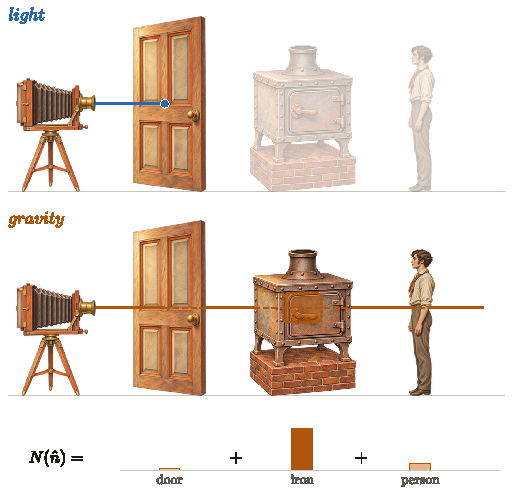
\includegraphics[width=\columnwidth]{figures/line-integral.pdf}
\caption{Two ways of forming a picture. A camera's line of sight passes
through a closed door, a closed iron furnace with a hot iron block inside, and
a person. In light it ends where it meets the door's face (the dot): a pixel
reports one point. Gravitational radiation passes through everything, so the
line runs on, dashed where a body hides it, and the hot block shows through the
furnace's walls. The pixel reports the sum along the whole line,
Eq.~\eqref{eq:column}: each body $k$ adds its number emissivity $j_{N,k}$ times
the length $\ell_k$ of the line inside it, shown below for illustrative
values in which the hot iron is far the brightest and the door, crossed only
through its thickness, adds little. The objects are illustrations, and their
sizes are chosen so that one level line crosses the middle of each.}\label{fig:line-integral}
\end{figure}

Figure~\ref{fig:closed-furnace} shows the first consequence at work. Two
closed steel furnaces hold the same block of iron, one at room temperature and
one at $1500\,\mathrm{K}$. They look the same and, to within the mass of their
heat ($\Delta U/c^2$, about $10^{-11}\,\mathrm{kg}$ per megajoule
\cite{Tolman1930}), weigh the same, so neither light nor the near field can
tell them apart at any ordinary sensitivity; the hot iron glows through the
steel. If the friction depended neither on frequency nor on temperature, the
number of gravitons emitted would grow as $T^3$ and the hot block would outshine
the cold one more than a hundredfold; the next paragraph explains why, for a
material whose stresses simply relax, this is an upper estimate.

\begin{figure*}
\centering
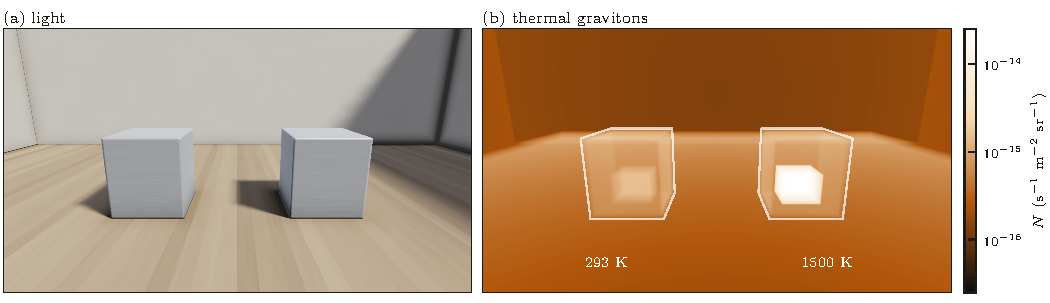
\includegraphics[width=\textwidth]{figures/closed-furnace.pdf}
\caption{The closed furnace, computed. Two closed steel furnaces
hold the same block of iron, one at $293\,\mathrm{K}$ and one at
$1500\,\mathrm{K}$. (a) Ordinary light: the two are identical. (b) The expected
thermal number radiance, Eq.~\eqref{eq:column}, from the same camera, on a
logarithmic scale, with the outlines that light shows. The hot iron glows
through its steel; the cold block cannot be told from its surroundings. The
room itself glows faintly, brightest where a line of sight crosses the floor
at a slant. The values assume the placeholder friction discussed in the
text.}\label{fig:closed-furnace}
\end{figure*}

\paragraph{Gravitational colour.} Equation~\eqref{eq:alpha} holds when the wave
is slower than the processes that produce viscosity. At the frequencies of heat
that is rarely so, and $\eta$ must be replaced by the dissipative part of the
material's shear response at the frequency of the wave, the real part of its
dynamic viscosity, $\mathrm{Re}\,\eta(\omega)$ \cite{BaymPatilPethick2017}. A
simple model shows how much this matters. A liquid whose stresses relax in a
time $\tau$ (Maxwell's model) has
\begin{equation}\label{eq:maxwell}
\mathrm{Re}\,\eta(\omega) = \frac{\eta_0}{1 + \omega^2\tau^2} ,
\end{equation}
so its everyday viscosity $\eta_0$ survives only below $\omega \approx 1/\tau$.
Above it the friction falls as $\eta_0/(\omega\tau)^2 = G_\infty^2/\eta_0\omega^2$,
where $G_\infty = \eta_0/\tau$ is the liquid's stiffness against sudden shear:
at a given stiffness, the more viscous liquid glows the less. Honey is viscous
because its molecules rearrange slowly; at the frequencies of heat that
rearrangement is frozen, and honey need not outshine water at all. In dense
matter the friction at those frequencies comes from much faster processes, and
an order-of-magnitude guess is $10^{-4}$ to $10^{-3}\,\mathrm{Pa\,s}$, which is
why we use $10^{-3}\,\mathrm{Pa\,s}$ as a placeholder. A crystal has no sound
waves above its Debye frequency, so above its Debye temperature its glow grows
more slowly than $T^3$ as well. Maxwell's model falls steadily with
frequency; a real material can have resonances in its losses, and then needs
its own spectrum of stress fluctuations, which may exceed this estimate in a
band. The spectrum of the glow therefore records a
material's mechanical losses, a kind of gravitational colour, and with a
frequency-dependent friction the number emissivity must be computed as
$j_N = \int \alpha(\omega)\,B_\omega\,\dd\omega/\hbar\omega$ rather than by
dividing the power by $2.70\,k_BT$.

Two consequences follow. The honey-and-water demonstration shows the contrast
that everyday viscosity would give, and is labelled as such. And temperature
cannot be read from the glow alone: a different temperature with a different
friction spectrum gives the same $j_\omega$, so a thermal gravitational image
measures temperature only when the material's response is known from elsewhere.

\paragraph{A glowing volume or a glowing outline?} Thermal radiation from the
vibrations of a solid has been calculated before
\cite{SchaeferDehnen1981,SchaeferDehnen1981erratum,DehnenRomeroSchaefer1984};
for an elastic sphere without internal damping its strength was found to grow
with the sphere's surface, not its volume. Which channel wins should depend on
how far a sound wave travels before it is damped: where that distance is much
shorter than the body, as in most solids at room temperature, the volume
emission of Eq.~\eqref{eq:kirchhoff} should dominate, while a cold, pure crystal
might glow at its surface. Both can be computed. In an elastic body without
loss a wave is absorbed only where the stiffness changes, at the surface, where
it launches sound \cite{Dyson1969}; for a sphere below its Debye temperature
the thermal glow that follows is \cite{DehnenRomeroSchaefer1984}
\begin{equation}\label{eq:surface-glow}
L_S = 4\pi R^2\,\frac{\pi^2}{24}\Bigl(1 + \frac{3c_T}{2c_L}\Bigr)
\frac{G\rho\,c_T^3\,(k_BT)^2}{\hbar c^5} ,
\end{equation}
with $c_T$ and $c_L$ the speeds of shear and compressional sound: by
Kirchhoff's law, a surface that absorbs the fraction
$\pi^2(1 + 3c_T/2c_L)\,G\rho c_T^3/c^3\omega^2$ of a wave, Dyson's absorption
with its constant. Friction inside, $\mathrm{Re}\,\eta = \rho c_T^2/\omega Q$ for
sound of quality factor $Q$, makes the volume glow by Eq.~\eqref{eq:kirchhoff},
with $L_V = V\,32\zeta(3)\,G\rho c_T^2 (k_BT)^3/\pi c^5 Q\hbar^2$, and
\begin{equation}\label{eq:volume-surface}
\frac{L_V}{L_S} = \frac{256\,\zeta(3)}{\pi^3\,(1 + 3c_T/2c_L)}\,
\frac{R}{\ell_s} ,
\end{equation}
where $\ell_s = Q\hbar c_T/k_BT$ is the distance a thermal phonon travels
before it is damped; the prefactor is $5.5$ for steel. Thermal phonons in
solids at room temperature travel nanometres, so ordinary bodies glow through
their volume: a steel ball of radius $10\,\mathrm{cm}$ at room temperature
glows $10^{-46}\,\mathrm{W}$ from its surface and, with $Q\approx10$ for its
thermal phonons, $7\times10^{8}$ times more from its volume. A pure crystal cooled until
its phonons cross it glows at its surface, in proportion to $T^2$ rather than
$T^3$, as Dehnen, Romero and Schäfer found. The reference implementation
checks both expressions by integrating Kirchhoff's law over the spectrum.
